\documentclass{article}
\usepackage[utf8]{inputenc}

\title{Queries}
\author{Benny Chen, Disha Verma, Joshua Lee, Alina Baby}
\date{\today}

\usepackage{color}
\usepackage{amsthm}
\usepackage{amssymb} 
\usepackage{amsmath}
\usepackage{listings}
\usepackage{xcolor}
\usepackage{listings}
\usepackage{graphicx}
\usepackage[hidelinks]{hyperref}

\definecolor{codegreen}{rgb}{0,0.6,0}
\definecolor{codegray}{rgb}{0.5,0.5,0.5}
\definecolor{codepurple}{HTML}{C42043}
\definecolor{backcolour}{HTML}{F2F2F2}
\definecolor{bookColor}{cmyk}{0,0,0,0.90}  
\color{bookColor}

\lstset{upquote=true}

\lstdefinestyle{mystyle}{
    backgroundcolor=\color{backcolour},   
    commentstyle=\color{codegreen},
    keywordstyle=\color{codepurple},
    numberstyle=\numberstyle,
    stringstyle=\color{codepurple},
    basicstyle=\footnotesize\ttfamily,
    breakatwhitespace=false,
    breaklines=true,
    captionpos=b,
    keepspaces=true,
    numbers=left,
    numbersep=10pt,
    showspaces=false,
    showstringspaces=false,
    showtabs=false,
}
\lstset{style=mystyle}

\newcommand\numberstyle[1]{%
    \footnotesize
    \color{codegray}%
    \ttfamily
    \ifnum#1<10 0\fi#1 |%
}

\begin{document}

\maketitle

\section*{Query 1}

The first query we made was to get a general overview of incidents from a certain customer from one destination to another (by zip code). This query shows the date, name, the description of what happened and the zip codes of the route. This would help with a consise report on the incident that happened from that route.
\begin{lstlisting}[ language=SQL,
    deletekeywords={IDENTITY},
    deletekeywords={[2]INT},
    morekeywords={clustered},
    framesep=8pt,
    xleftmargin=40pt,
    framexleftmargin=40pt,
    frame=tb,
    framerule=0pt ]
SELECT r.Report_Date, c.NAME, i.Description,
s.ZipCode AS Starting_location_ZipCode,
d.ZipCode AS Destination_ZipCode
FROM CUSTOMER c
INNER JOIN HOUSEHOLD_GOODS h ON c.CustomerID = h.CustomerID AND c.Starting_location_NO_ID = h.Starting_location_NO_ID
INNER JOIN Report r ON h.HouseholdGood_ID = r.HouseholdGood_ID
INNER JOIN INCIDENT i ON r.Incident_ID = i.Incident_ID
INNER JOIN `STARTING LOCATION` s ON h.Starting_location_NO_ID = s.Starting_location_NO_ID
INNER JOIN DESTINATION d ON r.Destination_NO_ID = d.Destination_NO_ID
WHERE c.NAME = 'Glenna Jarvis'
\end{lstlisting}

This outputs the following table:

\begin{center}
    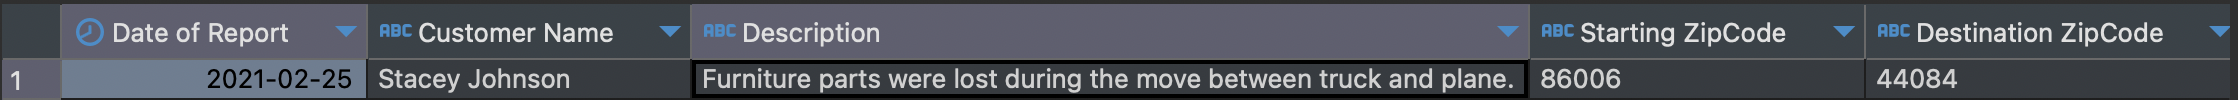
\includegraphics[width=0.9\textwidth]{./images/Q1.png}
\end{center}

\section*{Query 2}

The second query we aggregate the data to find those who have made unsuccessful payments. In this table we can see the name, policy type, customer ID, phone number, payment amount, and the number of days since due date. This would help with customer service as we can see who has made unsuccessful payments and contact them to see if they would like to make a repayment or cancel their policy. This is also ordered by the number of days since the due date so we can see who has been delinquent the longest and contact them first.

\begin{lstlisting}[ language=SQL,
    deletekeywords={IDENTITY},
    deletekeywords={[2]INT},
    morekeywords={clustered},
    framesep=8pt,
    xleftmargin=40pt,
    framexleftmargin=40pt,
    frame=tb,
    framerule=0pt ]
SELECT c.NAME AS 'Customer Name', 
po.Policy_Type AS 'Policy', 
c.CUSTOMERID AS 'Customer ID', 
c.PHONE_NUMBER AS 'Phone Number', 
p.Payment_Amount AS 'Payment Due',
DATEDIFF(NOW(), p.Payment_Date) AS 'Days Delinquent' 
FROM CUSTOMER c
INNER JOIN PAYMENT p ON c.CUSTOMERID = p.CustomerID
INNER JOIN POLICY po ON c.CUSTOMERID = po.CustomerID
WHERE p.Success_Status = 'Unsuccessful'
ORDER BY DATEDIFF(NOW(), p.Payment_Date) DESC;    
\end{lstlisting}

This outputs the following table:

\begin{center}
    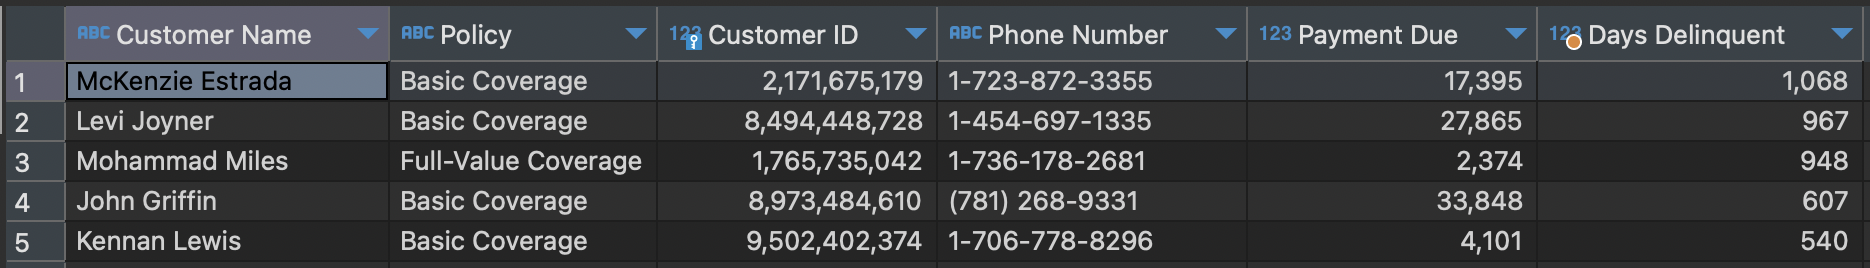
\includegraphics[width=0.9\textwidth]{./images/Q2a.png}
\end{center}

\section*{Query 3}

The third query we made was to filter the data by those who have been constantly using the service. This would show a company that this customer is a high risk customer. The filter narrows down those who have multiple reports and have only been using the service for a year. This would output all customers that fit this along with their name, policy, policy number, the number of reports, and the total number of goods. this would help catch fraud and help the company decide if they want to continue to do business with this customer.

\begin{lstlisting}[ language=SQL,
    deletekeywords={IDENTITY},
    deletekeywords={[2]INT},
    morekeywords={clustered},
    framesep=8pt,
    xleftmargin=40pt,
    framexleftmargin=40pt,
    frame=tb,
    framerule=0pt ]
SELECT C.NAME, P.Policy_Number, COUNT(R.Report_ID) AS Num_Reports, SUM(R.Quantity_of_Goods) AS Total_Goods
FROM CUSTOMER C
JOIN POLICY P ON C.CUSTOMERID = P.CustomerID
JOIN HOUSEHOLD_GOODS HG ON C.CUSTOMERID = HG.CustomerID
JOIN Report R ON HG.HouseholdGood_ID = R.HouseholdGood_ID
WHERE P.Policy_End_Date <= DATE_ADD(P.Policy_Start_Date, INTERVAL 1 YEAR)
GROUP BY C.NAME, P.Policy_Number
HAVING COUNT(R.Report_ID) > 1
ORDER BY Num_Reports DESC;
\end{lstlisting}

This outputs the following table:

\begin{center}
    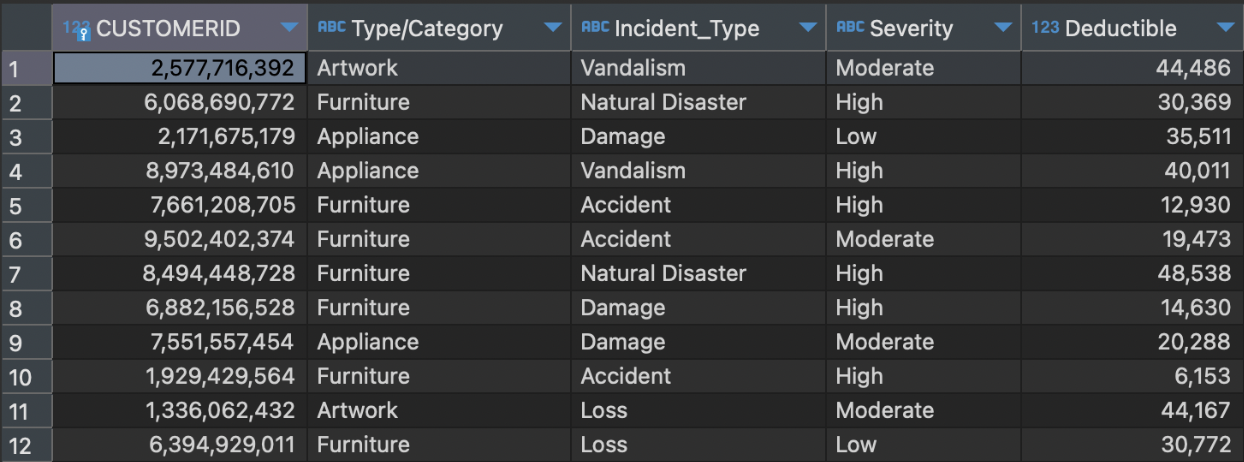
\includegraphics[width=0.9\textwidth]{./images/Q3.png}
\end{center}

\section*{Query 4}

In the fourth query we aggregate the data to find the departure and arrival times of the move along with how far it was. This would help with the company to see how long it takes to move a customer from one location to another depending on the distance and if that factor affects incidents that happen during the move. This query shows the CustomerID, name, the departure time, the arrival time, and the distance of the move.

\begin{lstlisting}[ language=SQL,
    deletekeywords={IDENTITY},
    deletekeywords={[2]INT},
    morekeywords={clustered},
    framesep=8pt,
    xleftmargin=40pt,
    framexleftmargin=40pt,
    frame=tb,
    framerule=0pt ]
SELECT 
c.CUSTOMERID, 
c.NAME, 
s.Depart_Date, 
d.Arrival_Date,
de.Travel_Distance_in_Miles
FROM 
CUSTOMER c 
JOIN HOUSEHOLD_GOODS h ON c.CUSTOMERID = h.CustomerID 
JOIN `STARTING LOCATION` s ON h.Starting_Location_NO_ID = s.Starting_location_NO_ID
JOIN Report r ON h.HouseholdGood_ID = r.HousholdGood_ID 
JOIN DESTINATION d ON r.Destination_NO_ID = d.Destination_NO_ID
JOIN DESTINATION de ON r.Destination_NO_ID = de.Destination_NO_ID;
\end{lstlisting}

This outputs the following table:

\begin{center}
    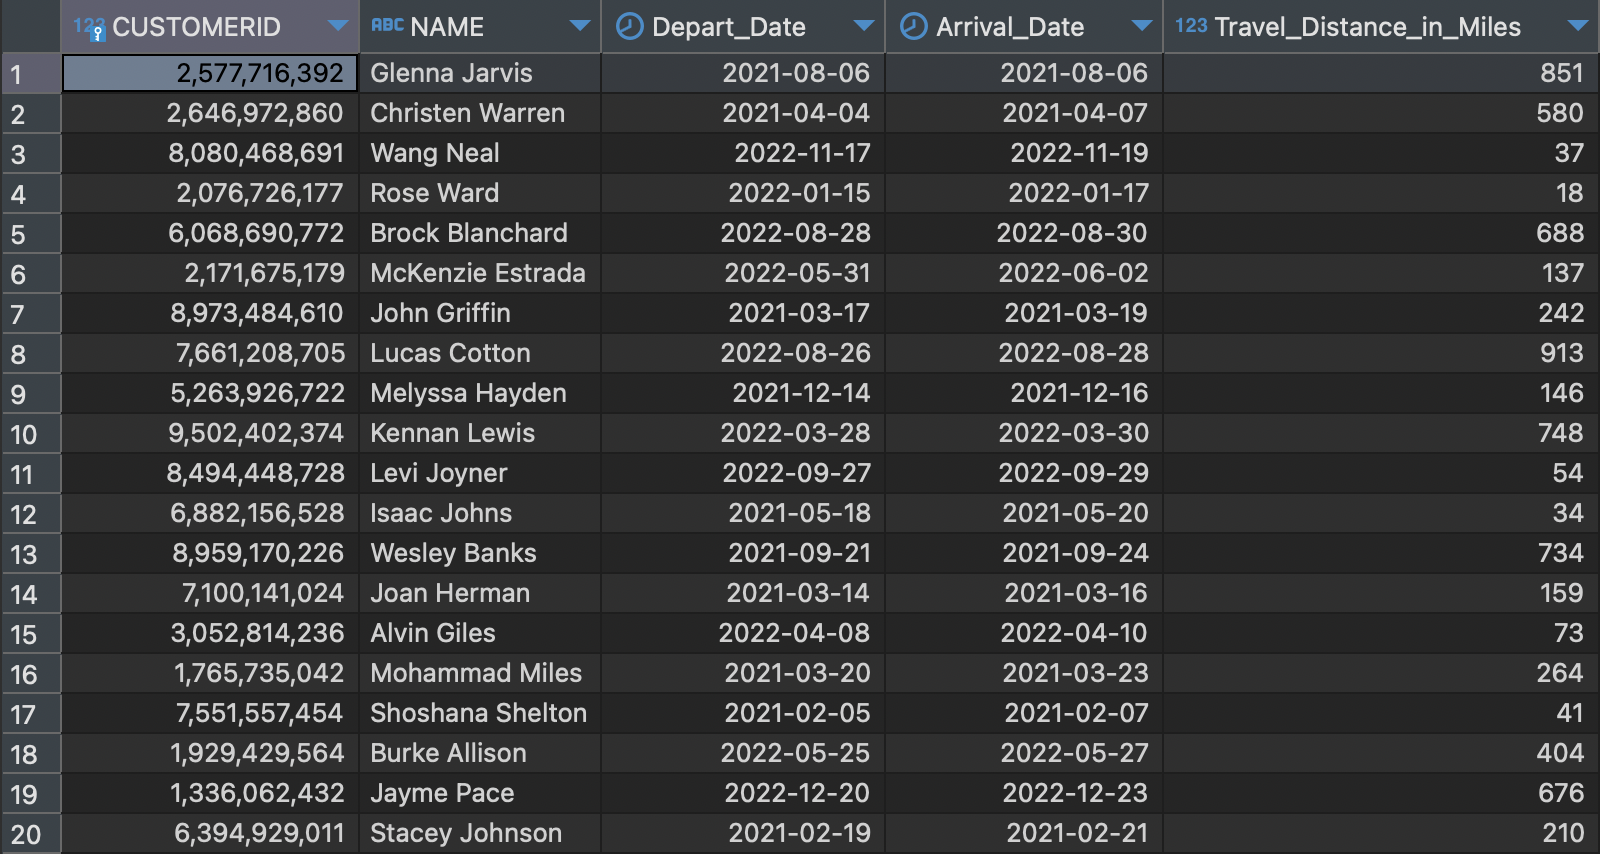
\includegraphics[width=0.9\textwidth]{./images/Q4.png}
\end{center}

\section*{Query 5}

In this query we filter the data by the year, in this case 2021, and output the number of cases and percentages of the number of incidents that happened in the year. This would help with the company to see what types of incidents happen the most and shape the insurance policy to better cover those incidents. This query shows the type of the insured, the number of cases of it that year, and the percentage as a whole.

\begin{lstlisting}[ language=SQL,
    deletekeywords={IDENTITY},
    deletekeywords={[2]INT},
    morekeywords={clustered},
    framesep=8pt,
    xleftmargin=40pt,
    framexleftmargin=40pt,
    frame=tb,
    framerule=0pt ]
SELECT H.`Type/Category` AS 'Type of Case', 
COUNT(H.`Type/Category`) AS 'Number of Cases', 
COUNT(H.`Type/Category`) * 100.0 / SUM(COUNT(H.`Type/Category`)) OVER() AS 'Percentage within Year'
FROM HOUSEHOLD_GOODS H
JOIN POLICY P ON H.CustomerID = P.CustomerID
JOIN Report R ON H.HouseholdGood_ID = R.HouseholdGood_ID
WHERE YEAR(R.Report_Date) = 2021
GROUP BY H.`Type/Category`;
ORDER BY 
\end{lstlisting}

This outputs the following table:

\begin{center}
    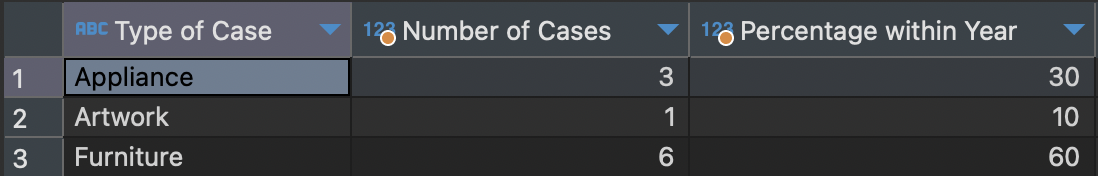
\includegraphics[width=0.9\textwidth]{./images/Q5.png}
\end{center}

%TODO make a query for most common zip code, most common policy and lest common, number of people ordered, and average deductible

\end{document}